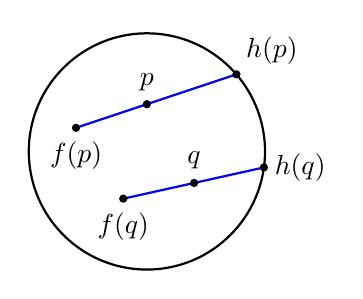
\begin{tikzpicture}
\draw[thick] (0,0) circle (1.5);
\draw[blue, thick] (-0.9,0.3) -- (1.137,0.979);
\draw[blue, thick] (-0.3,-0.6) -- (1.486,-0.203);
\foreach \p in {(-0.9,0.3),(0,0.6),(1.137,0.979),(-0.3,-0.6),(0.6,-0.4),(1.486,-0.203)} \fill \p circle (1.5pt);
\node[below] at (-0.9,0.25) {$f(p)$};
\node[above] at (0,0.65) {$p$};
\node[above right] at (1.137,0.979) {$h(p)$};
\node[below] at (-0.3,-0.65) {$f(q)$};
\node[above] at (0.6,-0.35) {$q$};
\node[right] at (1.5,-0.2) {$h(q)$};
\end{tikzpicture}
